\section{Criteri di stima}
% ######################################################################## Stima ai mimimi quadrati - last square - LS
\subsection{Stima ai mimimi quadrati - last square - LS}
\index{Stima ai minimi quadrati (LS)}
Innanzi tutto, un'importante premessa è che il numero delle osservazioni $N$ sia almeno pari al numero dei parametri $q$ da stimare, quindi deve valere $N\geq q$. Nel caso in cui $N>q$, allora non sarà possibile trovare un modello che spieghi esattamente i dati per via degli errori di misura, inoltre, la realtà non è mai perfettamente modellabile. Per chiarire questo concetto di seguito vengono presentati due grafici che rappresentano i due casi $N=q$ e $N>q$:
% GRAFICI DEI DUE CASI
\textbf{GRAFICO DA FARE, NON VIENE BELLO}
\begin{figure}[htbp]
  \centering
  %\subfigure[Il rango non è massimo, ci sono infiniti punti di minimo\label{fig:grafo3Dnomin}]{\includegraphics[keepaspectratio]{mathematica/intercaso1}}
  
  %\subfigure[Il rango è massimo e il punto di minimo è unico\label{fig:grafo3Dmin}]{\includegraphics[keepaspectratio]{mathematica/intercaso2}}
  
  \caption{Confronto fra modelli che hanno tanti parametri quanti i dati, e modelli che hanno un numero di dati maggiore al numero di parametri.\label{fig:confrontomodellidatiparametri}}
\end{figure}

Come si può vedere, nel caso $N>q$ abbiamo dovuto usare una retta di regressione che minimizzasse gli errori, ma non ci è possibile creare una retta che passi per tutti i punti. Dato che il caso $N>q$ è la norma, e quindi non ci è possibile creare modelli esatti, ci "accontentiamo" che i residui\index{Residuo} \footnote{il residuo è l'errore commesso dal modello rispetto ad un particolare dato} siano piccoli $\varepsilon$ sia piccolo:

  \[ \varepsilon :=Y-\Phi(u)\cdot \theta \]
  
A esempio, potremmo desiderare che la somma dei quadrati dei residui sia piccola -SSR\footnote{Sum of Square Residual}- \index{Somma dei quadrati dei residui, Sum of Square Residual (SSR)} sia piccola:

  \[ SSR=\sum_{i=1}^{N}{\varepsilon_i^2 } = {||\varepsilon ||}^2 = (Y-\Phi(u)\cdot \theta)^T \cdot (Y-\Phi(u)\cdot \theta) \]
  
D'ora in avanti, per brevità, $\Phi\equiv \Phi(u)$. Il nostro interesse ora è trovare i parametri $\theta$ che minimizzino l'errore quadratico.
\paragraph{Teorema} supponendo che $rank[\Phi]=q$\footnote{ovvero che il rango della matrice di sensitività $\Phi$ sia pari a $q$, quindi che il numero di colonne linearmente indipendenti di $\Phi$ sia pari al numero di variabili $q$}, allora $ J(\theta):={||\varepsilon ||}^2 $ ha un minimo globale in corrispondenza di:
  \[ \theta=(\Phi^T\Phi)^{-1}\cdot \Phi^TY \]
Prima di procedere alla dimostrazione di questo teorema, si veda l'appendice \ref{app:operatorimatriciali}


\begin{dimostrazione}

  \[ rank[\Phi]=q \Longrightarrow det(\Phi^T\Phi) \ne 0 \]
  
se, per assurdo, $det(\Phi^T\Phi)=0$

  \[ 
    \begin{split}
      \exists x \ne 0 | \Phi^T\Phi x=0 &\Longrightarrow x^T\Phi^T\Phi x=0 \Longrightarrow ((\Phi x)^T\Phi x)=\| \Phi x \|^2 =0 \Longrightarrow \Phi x =0\\
       &\Longrightarrow rank[\Phi]<q \Longrightarrow \text{assurdo!} \Longrightarrow \exists (\Phi^T\Phi)^{-1} 
    \end{split} 
  \]
  
Ora che abbiamo verificato l'esistenza della matrice inversa, calcoliamo il gradiente dell'errore per cercare di minimizzarlo.

  \begin{gather*}
    J(\theta)=\varepsilon^T\varepsilon=(Y-\Phi\theta)^T(Y-\Phi\theta)\\
    \frac{dJ(\theta)}{d\theta}=2(Y-\Phi\theta)^T\Phi
  \end{gather*}
  
Vogliamo che $J(\theta)$ sia minimo per cui calcoliamo il valore del vettore $\theta$ che annulla il gradiente:

  \[ 
    \begin{split}\frac{dJ(\theta)}{d\theta} = 0 &\Leftrightarrow  2(Y-\Phi\theta)^T\Phi=Y^T-\theta^T\Phi^T=0 \Leftrightarrow Y^T\Phi=\theta^T\Phi^T\Phi \\ &\Leftrightarrow \Phi^TY=\Phi^T\Phi\theta \Leftrightarrow \theta= (\Phi^T\Phi)^{-1}\Phi^TY 
    \end{split}
  \]
  
Quello che abbiamo calcolato è un punto di massimo o minimo, per cui ora verifichiamo che sia di minimo calcolando la sua derivata seconda, se risulterà maggiore di zero allora sarà un minimo.

  \[ 
    \begin{split} \frac{d^2J(\theta)}{d\theta^2}&=\frac{d}{d\theta}\{\frac{dJ(\theta)}{d\theta}\}= \frac{d}{d\theta}\{2(Y-\Phi\theta)^T\Phi\}=2\frac{d}{d\theta}\{(Y-\Phi\theta)^T\}\Phi\\
  &=2\frac{d}{d\theta}\{Y^T-\theta^T\Phi^T\}\Phi=2\Phi^T\Phi 
    \end{split} 
  \] 
  
%FIXME che fine fa il - nella formula?
\begin{center}[FIXME: che fine fa il meno nella formula? Penso sia dovuto al penultimo passaggio, applicando T forse doveva andare via]\end{center}

Essendo il risultato una diade:

  \[ D=\Phi^T\Phi \geq 0 \Longrightarrow \frac{d^2J(\theta)}{d\theta^2}=2D \geq 0 \]
  
Come volevasi dimostrare, è un punto di minimo
\end{dimostrazione}

Possiamo quindi concludere che la stima LS è definita come:

  \[ \theta^{LS}=\arg \min_{\theta} J(\theta) \]
  
che, come abbiamo dimostrato, corrisponde a:

  \[ \theta^{LS}=(\Phi^T\Phi)^{-1}\Phi^TY \]

Il teorema appena dimostrato può anche essere interpretato geometricamente. Prendiamo il caso di soli due parametri e quindi $q=2$

\begin{figure}[htbp]
  \centering
  \subfigure[Il rango non è massimo, ci sono infiniti punti di minimo\label{fig:grafo3Dnomin}]{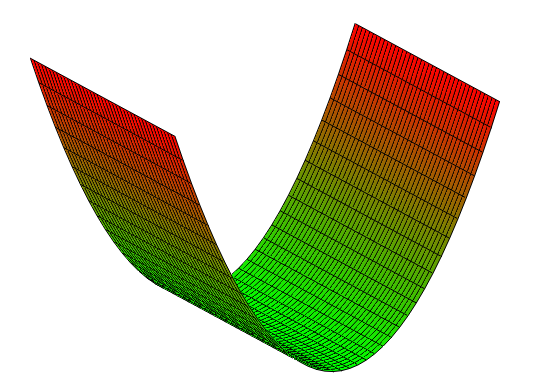
\includegraphics[scale=0.30]{img/graf3D1.png}}
  \subfigure[Il rango è massimo e il punto di minimo è unico\label{fig:grafo3Dmin}]{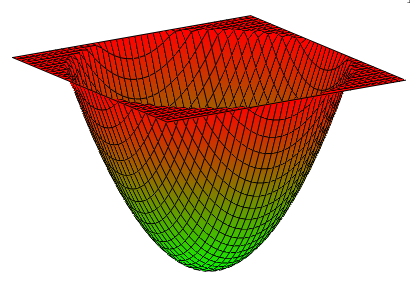
\includegraphics[scale=0.35]{img/graf3D2.png}}
  \caption{Identificabilità della soluzione\label{fig:identificabilitasoluzione}}
\end{figure}


Dati i grafici in figura \ref{fig:identificabilitasoluzione} vediamo nel grafico in figura \ref{fig:grafo3Dnomin} l'esempio in cui non si ha il rango massimo, infatti esistono infiniti punti di minimo. Nel grafico in figura \ref{fig:grafo3Dmin}, invece, abbiamo rango massimo ed un solo punto di minimo, quindi la soluzione si trova nel punto di minimo.\newline
Il problema studiato sin ora, ha fatto uso della supposizione che $rank[\Phi]=q\Rightarrow det(\Phi^T\Phi)\ne 0$, ma se così non fosse, abbiamo appena visto che si pone un problema di identificabilità\index{identificabilità}, ovvero, la soluzione non è unica come in figura \ref{fig:grafo3Dnomin}. Come scegliere la soluzione fra le infinite possibili? Supponiamo $q=3$ e che $rank[\Phi]=2$, quindi $rank[\Phi]<q$:

  \begin{gather*}
    \theta = \begin{bmatrix} \theta_1 \\ \theta_2 \\ \theta_3 \end{bmatrix}\quad
    \Phi=\begin{bmatrix} u_1(1) & u_2(1) & u_3(1) \\ u_1(2) & u_2(2) & u_3(2) \\ \vdots & \vdots & \vdots \\ u_1(N) &u_2(N) & u_3(N) \end{bmatrix}\\
    y(i)=\theta_1u_1(i)+\theta_2u_2(i)+\theta_3u_3(i)
  \end{gather*}
  
dato che $rank[\Phi]=2$, allora sappiamo che una colonna di $\Phi$ è linearmente dipendente dalle altre. Supponendo che la colonna dipendente sia quella associata a $u_3$ potremmo scriverla come:
  \[ u_3(i)=au_1(i)+bu_2(i) \]
dove i coefficienti $a$ e $b$ sono noti. Da qui possiamo scrivere:
  \[ y(i)=\theta_1u_1(i)+\theta_2u_2(i)+\theta_3(au_1(i)+bu_2(i)) = u_1(i)(\theta_1+a\theta_3)+u_2(i)(\theta_2+b\theta_3) \]
con questa riscrittura la variabile $u_3$ risulta inutile, potremmo quindi ridurre le matrici a:

    \[
      \bar{\theta} = \begin{bmatrix} \bar{\theta}_1 \\ \bar{\theta}_2 \end{bmatrix}= \begin{bmatrix}\theta_1+a\theta_3 \\ \theta_2+b\theta_3 \end{bmatrix} \quad
      \Phi=\begin{bmatrix} u_1(1) & u_2(1)  \\ u_1(2) & u_2(2)  \\ \vdots & \vdots  \\ u_1(N) &u_2(N) ) \end{bmatrix}
    \]
    
Risolvendo il modello per $\bar{\theta}$ ci siamo riportati nel caso $rank[\Phi]=q$ e quindi possiamo risolverlo come visto in precedenza ed avremo una soluzione unica data da:

  \[ \bar{\theta}^{LS}=\begin{bmatrix} \bar{\theta}_1^{LS} \\ \bar{\theta}_2^{LS} \end{bmatrix}=(\Phi^T\Phi)^{-1}\cdot \Phi^TY \]
  
Quali sono i casi in cui può capitare di avere $rank[\Phi]<q$?

  \begin{itemize}
    \item ingressi fissati
    \begin{itemize}
      \item modello sovraparametrizzato rispetto al fenomeno da descrivere; ad esempio l'uso di due variabili indipendenti ma con lo stesso effetto sulla variabile dipendente
      \item modello sovraparametrizzato rispetto all'informazione contenuta nei dati; ad esempio variabili dipendenti da altre
    \end{itemize}
    \item ingressi manipolabili
    \begin{itemize}
      \item se si usano più variabili per rendere più ricco di informazioni il modello
    \end{itemize}
  \end{itemize}
  
% ######################################################################## Stima ML
\subsection{Stima ML}
\index{Stima ML}
Per poter usare questo stimatore, occorre fare delle ipotesi sulla ddp dell'errore di misura. L'ipotesi fatta è che l'errore di misura $V$ abbia un andamento di tipo gaussiano:

  \[ V:=Y-\Phi\cdot\theta\quad
    V=\begin{bmatrix} V_1 \\ \vdots \\ V_N  \end{bmatrix}\quad
    V\sim N(0,\Sigma_V) , \Sigma_V>0 
  \]
  
Sotto l'ipotesi appena enunciata, con $rank[\Phi]=q$, se, inoltre, gli errori hanno tutti la stessa varianza $\Sigma_V=\sigma^2I$, allora valgono:

  \begin{align*}
    J^{ML}(\theta)&=\varepsilon ^T \Sigma_V^{-1}\varepsilon = \sum_{i=1}^{N}{\frac{\varepsilon_i^2}{\sigma_i^2} }\\
    \theta^{ML}&= \arg \max_{\theta} J^{ML}(\theta)=(\Phi^T\Sigma_V^{-1}\Phi)^{-1}\Phi^T\Sigma_V^{-1}Y=C \cdot Y\\
    E[{\theta^{ML}}]&=\theta \\
    Var[\theta^{ML}]&=(\Phi^T\Sigma_V^{-1}\Phi)^{-1}
  \end{align*}
  

\begin{dimostrazione} %###########
Dimostriamo la non polarizzazione dello stimatore:

  \[ E[\theta^{ML}]=E[CY]=C\cdot E[Y]=C\cdot E[\Phi\theta+V]=C\cdot E[\Phi\theta]+C\cdot E[V] \]
  
Sotto le ipotesi enunciate $E[V]=0$, quindi:

  \[ C\cdot E[\Phi\theta]+C\cdot E[V]=C\cdot E[\Phi\theta]=E[C\Phi\theta]=E\left[(\Phi^T\Sigma_V^{-1}\Phi)^{-1}\Phi^T\Sigma_V^{-1}\Phi\cdot\theta \right] \]
  
dato che $A^{-1}\cdot A=I$, ne consegue:

  \[ E\left[(\Phi^T\Sigma_V^{-1}\Phi)^{-1}\Phi^T\Sigma_V^{-1}\Phi\cdot\theta \right]=E[I\theta]=\theta \]
\end{dimostrazione}
\begin{dimostrazione} % ###########
Dimostriamo il risultato della varianza:
  \[ Var[\theta^{ML}]=Var[CY]=C\cdot Var[Y]\cdot C^T = C\cdot Var[\Phi\theta+V]\cdot C^T \]
dato che $\Phi\theta$ non è una V.C., non concorre a determinare la varianza, quindi:

  \[ 
  \begin{split}
      C\cdot Var[\Phi\theta+V]\cdot C^T&=C\cdot Var[V]\cdot C^T=C\Sigma_VC^T\\
      &=(\Phi^T\Sigma_V^{-1}\Phi)^{-1}\Phi^T\Sigma_V^{-1}\Sigma_V \Sigma_V^{-1} \Phi(\Phi^T\Sigma_V^{-1}\Phi)^{-1}\\
      &=(\Phi^T\Sigma_V^{-1}\Phi)^{-1}\Phi^T \Sigma_V^{-1} \Phi(\Phi^T\Sigma_V^{-1}\Phi)^{-1}\\
      &=(\Phi^T\Sigma_V^{-1}\Phi)^{-1}(\Phi^T \Sigma_V^{-1} \Phi)(\Phi^T\Sigma_V^{-1}\Phi)^{-1}=(\Phi^T\Sigma_V^{-1}\Phi)^{-1}
  \end{split} 
  \]
\end{dimostrazione}

Se, invece, sempre sotto l'ipotesi enunciata con $rank[\Phi]=q$, non avessimo la stessa varianza sugli errori, ma avessimo $\Sigma_V=\sigma^2\psi$, con $\sigma^2$ scalare incognito e $\psi$ matrice nota, allora:

  \begin{align*}
    \theta^{ML}&=(\Phi^T\frac{1}{\sigma^2}\psi^{-1}\Phi)^{-1}\Phi^T\frac{1}{\sigma^2}\psi^{-1}Y  =(\Phi^T\psi^{-1}\Phi)^{-1}\Phi^T\psi^{-1}Y  \\
    (\sigma^2)^{ML}&=\frac{1}{N}\{ (Y-\Phi\theta^{ML})^T\psi^{-1}(Y-\Phi\theta^{ML})\}=\frac{J_\psi^{ML}(\theta^{ML})}{N}\\
    J_\psi^{ML}&=\varepsilon ^T(\theta)\psi^{-1}\varepsilon (\theta)
  \end{align*} % nell'ultima formula non dovrebbe esserci anche \frac{1}{\sigma^2}
Da notare che $(\sigma^2)^{ML}$ è polarizzato e quindi per avere una stima non polarizzata bisogna usare:

  \[ (\sigma^2)^{ML}=\frac{J_\psi^{ML}(\theta^{ML})}{N-q} \]
  
\paragraph{Osservazione} La stima ML è meno sensibile alla presenza degli outlier rispetto alla stima MS come mostrato in figura \ref{fig:MLMSoutlier}

\begin{figure}[htbp]
  \centering
  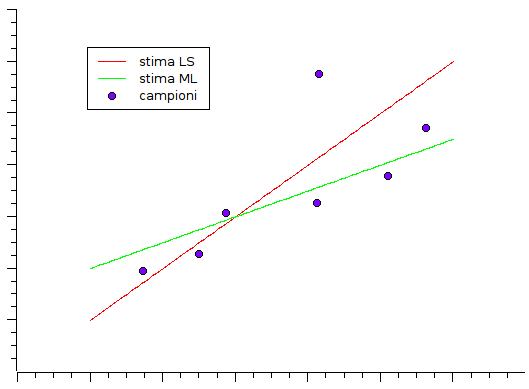
\includegraphics[scale=0.5]{img/outlier.png}
  \caption{Sensibilità delle stime ML e MS in presenza di outlier\label{fig:MLMSoutlier}}
\end{figure}

% ######################################################################## Intervalli di confidenza
\subsection{Intervalli di confidenza}
\index{Intervallo di confidenza}
Come già detto, fornire una stima senza dare informazioni sulla sua precisione è poco indicativo, vediamo quindi come calcolare l'intervallo di confidenza per la stima ML. Come visto dallo studio della stima ML ci son due casi: il primo dove l'errore di misura ha sempre la stessa varianza, quindi $\Sigma_V$ è una matrice nota; il secondo quando $\Sigma_V$ non è completamente nota ($\sigma^2$ è uno scalare sconosciuto e $\psi$ è una matrice nota).
Nel primo caso:

\begin{gather*}
    \theta^{ML}\sim N(\theta,\Sigma_{\theta^{ML}})\\
    I_\gamma(\theta_i)=\left[ \theta_i^{ML} - z_0\cdot\sigma_{\theta_i^{ML}}  ,  \theta_i^{ML} + z_0\cdot\sigma_{\theta_i^{ML}}\right]\quad \text{dove} \quad \sigma_{\theta_i^{ML}}^2 = \left[ \Sigma_{\theta^{ML}}\right]_{ii}\\
    z_0 | P(\left| Z \right| \leq z_0 ) =\gamma
\end{gather*}

nel secondo caso:

\begin{gather*}
  \Sigma_{\theta^{ML}}=\sigma^2(\Phi^T\psi^{-1}\Phi)^{-1}\\
  \frac{\theta_i^{ML}-\theta_i}{\hat{\sigma}_{\theta_i^{ML}}} \sim T_{N-q}\quad\text{dove}\quad\sigma_{\theta_i^{ML}}^2 = \left[ \Sigma_{\theta^{ML}}\right]_{ii}\\
  I_\gamma(\theta_i)=\left[ \theta_i^{ML} - t_0\cdot\sigma_{\theta_i^{ML}}  ,  \theta_i^{ML} + t_0\cdot\sigma_{\theta_i^{ML}}\right]\\
  t_0 | P(\left| T_{N-q} \right| \leq t_0 ) =\gamma
\end{gather*}

\begin{center} \rule{300pt}{1pt} \end{center}
\begin{esempio}
Applichiamo la regressione lineare. Supponiamo di avere:

  \[ y(t)=\theta_1u_1(t)+ \dots +\theta_qu_q(t)+v(t) \]

Se la distribuzione dell'errore è di tipo gaussiano, allora la stima ML coincide con la stima LS e quindi $\Sigma_V=I$. Nel modello riconosciamo le seguenti matrici:

  \[ \Phi(u)\begin{bmatrix} u_1(1) & u_2(1) & \dots & u_q(1) \\ u_1(2) & u_2(2) & \dots & u_q(2)\\ \vdots & \vdots & \dots & \vdots \\ u_1(N) & u_2(N) & \dots & u_q(N) \end{bmatrix}=\begin{bmatrix} \varphi(1)^T \\  \varphi(2)^T \\ \vdots \\ \varphi(N)^T \end{bmatrix} \]

dove con $\varphi$ viene indicato il vettore di regressione. Dato che nel caso gaussiano i due metodi di stima sono uguali:
\begin{center}
  $\theta^{ML}=\theta^{LS}=(\Phi^t\Phi)^{-1}\Phi^TY=\sum_{i=1}^{N} \varphi(i) y(i)$
\end{center}
Se è soddisfatta la condizione di identificabilità $rank[\Phi]=q$
\begin{center}
  $(\sigma^2)^{ML}=\frac{J(\theta^{ML})}{N-q}=\frac{\sum_{i=1}^{N} \varepsilon^2(t) }{N-q}=\frac{\sum_{i=1}^{N} {\left(y(i)-\varphi(i)^T\theta^{ML}\right)^2}}{N-q}$\newline
  $\Sigma_{\theta^{ML}}=(\sigma^2)^{ML}(\Phi^T\Phi)^{-1}=(\sigma^2)^{ML} { (\varphi(i) \varphi^T(i) )^{-1}}$
\end{center}
Da qui il risultato finale:
\begin{center}
  $y(t)=\theta_1^{ML}u_1(t)+ \dots +\theta^{ML}_qu_q(t)+\varepsilon (t)$\newline
  $\varepsilon (t)=y(t)-\varphi^T(t)\theta^{ML}$
\end{center}
Da notare, in conclusione, che per ogni parametro stimato vi sarà una varianza associata da usarsi per la determinazione degli intervalli di confidenza.
\end{esempio}
\begin{center} \rule{300pt}{1pt} \end{center}
